\documentclass[border=10pt,tikz]{standalone}
\usepackage{tikz}
\usetikzlibrary{positioning,arrows.meta}
\begin{document}
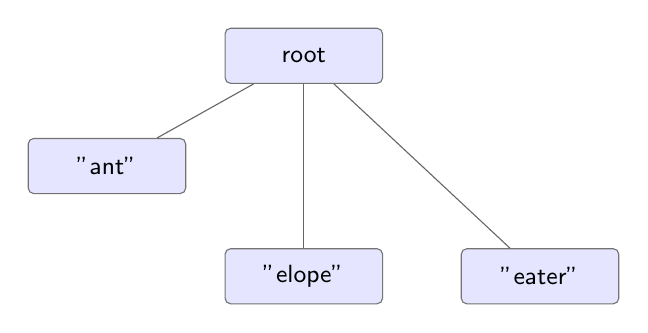
\begin{tikzpicture}[
  font=\sffamily\small,
  node/.style={rectangle, rounded corners=2pt, draw=black!55, line width=0.4pt,
               minimum height=7mm, minimum width=20mm, inner sep=2pt, fill=blue!10, align=center},
  edge/.style={draw=black!60, line width=0.4pt}
]
\node[node] (r)  at (0, 2)    {root};
\node[node] (ant) at (-2.5, 0.6) {"ant"};
\node[node] (e1)  at (0, -0.8)  {"elope"};
\node[node] (e2)  at (3, -0.8)  {"eater"};

\draw[edge] (r) -- (ant);
\draw[edge] (r) -- (e1);
\draw[edge] (r) -- (e2);
\end{tikzpicture}
\end{document}
